\chapter{Системный анализ предметной области и постановка задачи }
\section{Предметная область}
Существует конкурс КИО - «Конструируй, Исследуй, Оптимизируй» (рис. ~\ref{KIOemblem}). Он был создан 9 лет назад. Данный конкурс проводится для учеников с 1 по 11 класс. Существует три уровня: 
 \begin{itemize}
        \item начальный уровень - для учеников начальных классов,
        \item уровень I - для учеников от 5 до 7 класса включительно,
        \item уровень II - для старших участников. 
    \end{itemize}


\begin{figure}[h]
\begin{minipage}[h]{0.49\linewidth}
\center{
\includegraphics[width=0.5\linewidth]{KIOemblem1} \\ а)}
\end{minipage}
\hfill
\begin{minipage}[h]{0.49\linewidth}
\center{
\includegraphics[width=0.5\linewidth]{KIOemblem2} \\ б)}
\end{minipage}
\caption{Эмблемы конкурса КИО}
\label{KIOemblem}
\end{figure}

Участникам каждого уровня предлагаются три логические задачи. Все задачи отражают недавно возникшее направление научных исследований, которое, применительно к разным наукам, получило названия компьютерной математики, компьютерной физики, компьютерной биологии и т. д. За каждым игровым сюжетов стоит серьёзная и, возможно, ещё не решённая в общем виде задача, которая после окончания Конкурса подробно и популярно обсуждается на страницах журнала «Компьютерные инструменты в школе».
Задания конкурса представлены в форме компьютерных моделей-лабораторий с игровыми элементами. В процессе работы с заданием участник конструирует частичные решения задачи, которые оцениваются по установленным в задании критериям. Таким способом формируется «рекорд» - число или набор чисел, характеризующие степень достижения поставленных в задании целей. Механизм рекорда позволяет участникам оценивать собственное продвижение в решении задач, а для жюри конкурса рекорды являются основой для составления рейтинга. 
Конкурс позволяет ребятам из самых отдаленных уголков России участвовать наравне с ребятами из больших городов, если у них есть Интернет или электронная почта. 
По окончании Конкурса каждый участник получает электронный сертификат, заверенный электронной подписью. Это означает, что выдаваемый жюри Конкурса электронный сертификат зашифрован так, что его можно проверить на подлинность открытием в программе «Электронный сертификат» на сайте Конкурса, но подделать его невозможно.
Я учавствовал в создании Конкурса КИО-2010. Я создал логическую задачу "Прожорливый тьюрмит". Для меня это был бесценный опыт, и я с радостью учавствую в модернизации Конкурса сейчас. Созданная мною игра будет описана в примерах задач.
Далее приведены примеры задач.
\subparagraph{Прожорливый тьюрмит (рис. ~\ref{ant}}
Существо, которое в теории алгоритмов называют тьюрмитом (Тьюринг+термит), перемещается по тору, развертка которого представлена в виде клетчатого поля 20x20. Тор, который мы может представить в виде бублика, получится из этого поля, если его «свернуть в трубочку», а затем соединить края трубки. При этом соседними станут верхние и нижние клетки каждого столбца и каждой строки исходного поля.

Управляется тьюрмит автоматом, графическое  изображение которого находится справа. Каждый кружок представляет собой состояние, в котором находится в данный момент «мозг» тьюрмита, а стрелочки между состояниями соответствуют действиям тьюрмита в той или иной ситуации.

Всего ситуаций, по которым «мозг» тьюрмита принимает решения, две – есть ли яблоко перед ним или нет. В каждой из ситуаций тьюрмит может совершить три действия: пойти прямо и перейти в следующую клетку, повернуться вправо или влево. Если в клетке, в которую попадает тьюрмит, находится яблоко, то он съедает его.

Ваша  задача состоит в том, чтобы сконструировать  такой «мозг» тьюрмита, который позволит ему за 130 шагов съесть как можно больше яблок. При одинаковом числе съеденных яблок лучшей считается та конструкция автомата, которая имеет меньшее число состояний. Обратите внимание на то, что тьюрмит может сделать много шагов, находясь в одном состоянии. В этом случае автомат будет иметь петлю, начинающуюся и заканчивающуюся в этом состоянии.
\begin{figure}[!ht]
	\begin{center}
		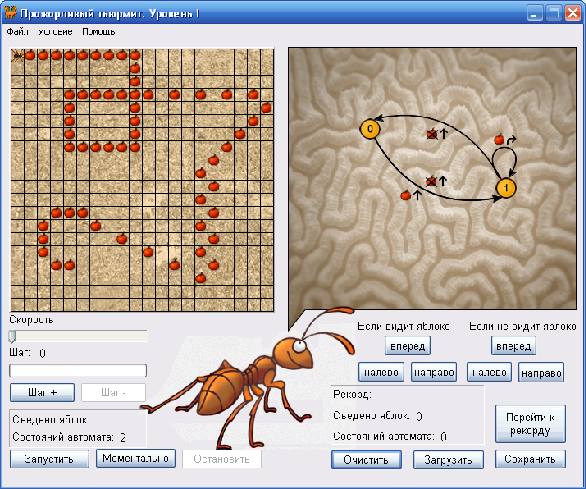
\includegraphics[]{ant}
	\end{center}
	\caption{Прожорливый тьюрмит}
	\label{ant}
\end{figure}


\subparagraph{Освещение города.}
Демонстрация полностью настраиваемых окружений типа <<теорема>>.
Муниципалитет маленького городка хочет сэкономить на освещении улиц. Помогите ему разработать схему освещения, расставив фонари так, чтобы они осветили все закоулки города, но число фонарей при этом было минимальным (рис. ~\ref{town_light1}).
\begin{figure}[!ht]
	\begin{center}
		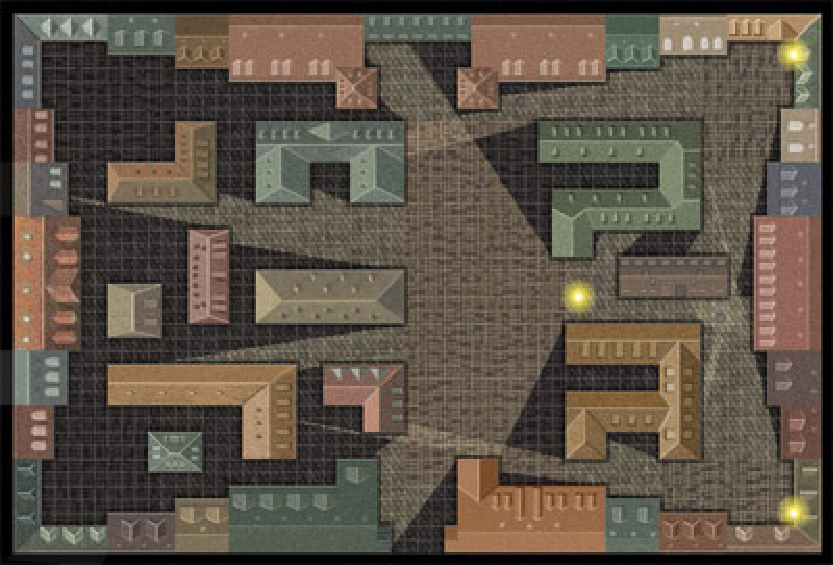
\includegraphics[]{town_light1}
	\end{center}
	\caption{Освещение города}
	\label{town_light1}
\end{figure}

\subparagraph{Сезам, откройся!}
От каждого путника, желающего добыть новое сокровище горы Сезам, Дух Горы требует принести несколько серебряных монет. По своему усмотрению Дух обращает часть монет в золотые монеты желтого золота, а остальные - в монеты красного золота, которые немного тяжелее монет из желтого золота. При этом Дух никогда не превращает все монеты в золотые одного вида. Путника, принесшего монеты, Дух испытывает задачей. Он просит не более четырёх раз положить равное число монет на разные чашки весов так, чтобы после превращения монет в золотые равновесие весов хотя бы раз нарушилось. При этом хитрый Дух всегда старается так превращать монеты в два вида золотых, чтобы при всех взвешиваниях весы оставались в равновесии. Вы должны перехитрить Духа и указать такой алгоритм взвешиваний, при котором для выбранного вами числа монет равновесие всегда нарушается (рис. ~\ref{open_sesame}).
\begin{figure}[!ht]
	\begin{center}
		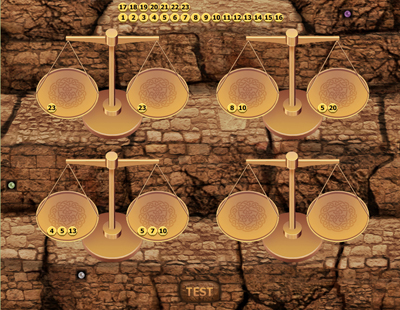
\includegraphics[]{open_sesame}
	\end{center}
	\caption{Сезам, откройся}
	\label{open_sesame}
\end{figure}
\subparagraph{Математическое скалолазание.}
Известно, что многие известные ученые занимались альпинизмом. Однажды они устроили соревнование по скалолазанию по необычным правилам. Одна команда забивает в скалу 16 крючьев, а другая соединяет крючья веревкой без пересечений так, чтобы потом как можно скорее пройти по ней весь маршрут. Считается, что по всем участкам маршрута скалолазы движутся с одной скоростью, поэтому вторая команда всегда прокладывает веревку по крючьям так, чтобы минимизировать длину маршрута. Наоборот, команда, забивающая крючья, должна позаботиться о том, чтобы даже самый короткий маршрут, проложенный по ним, был как можно длиннее. Ваша задача – вбить крючья так, чтобы максимально усложнить задачу сопернику(рис. ~\ref{rock_climber1}).
\begin{figure}[!ht]
	\begin{center}
		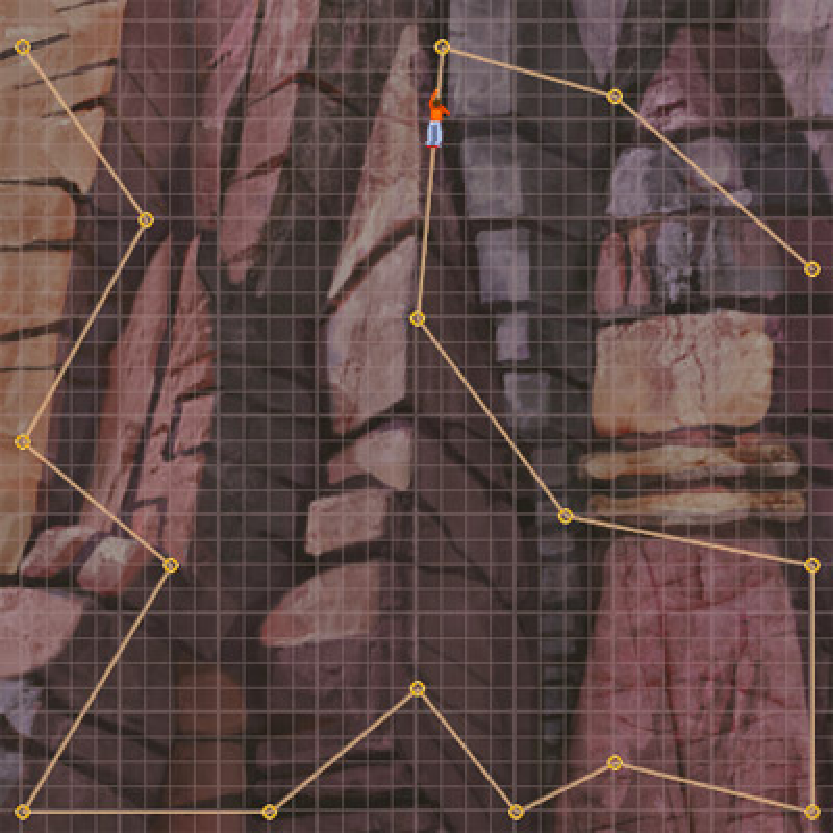
\includegraphics[]{rock_climber1}
	\end{center}
	\caption{Математическое скалолазание}
	\label{rock_climber1}
\end{figure}

До 2011 года все задачи создавались на языке Delphi. Начиная с 2011 года задачи стали делать на Flash. Flash — удобная кроссплатформенная среда для создания проектов. Так как во многих школах России теперь устанавливается СПО — свободное программное обеспечение, и, соответственно, ставится Unix подобные системы, то конкурс в виде exe-файла перестал быть легкодоступен для всех желающих участников. Для Flash-приложений же достаточно лишь наличие браузера и Flash Player'а. В этом году появилась возможность использовать динамическую библиотеку, созданную в ИТМО, которая позволяет облегчить серьёзные математические вычисления, которые приходится производить при создании подобных проектов. Возникла проблема в том, что Flash не может напрямую использовать динамические библиотеки. 


\section{Постановка задачи дипломного проекта}
При создании различных приложений часто требуются математические и другие пакеты, которые уже реализованы в виде динамических библиотек, и создавать их заново, используя, например, Flash, слишком затратно. То есть существует потребность использовать из Flash-приложений уже имеющиеся динамические библиотеки. Решение данной проблемы касается не только FLash-приложений, а любых других платформ, используемых для создания клиентской части веб-приложения (Javascript, SilverLight, PHP, Python, Ruby).
Напрямую из Flash нет возможности обращаться к динамическим библиотекам. Цель диплома - разработать компоненты, которые позволили бы использовать динамический библиотеки из Flash.
Если был бы доступен исходных код библиотек, то можно было бы его адаптировать к вызову из Flash. В данном случае это будет неуниверсальный способ и при любых изменениях в динамической библиотеке, адаптацию придётся проводить заново. Нужно найти универсальный способ, который будет работать при подключении любой динамической библиотеки.
Требованию к разрабатываему продукту:
\begin{itemize}
  \item Время на вызов функции через созданные в дипломе модули не должно отразиться на общей скорости приложения. Замедление работы программы не должно быть заметно ползователю;
  \item Весь проект должен занимать как можно меньше места, так как его будут скачивать участники со всех уголков России, у которых пропускная способность интернет-канала может быть слишком слабой для больших файлов. То есть увеличение размера не должно превышать нескольких мегабайт.
  \item Проект должен работать как под Windows, так и в различных дистрибутивах Linux;
  \item Из динамической бибилиотеки требуется вызывать функции. Каждая функция задаётся ее именем, типом возврщаемого значения, и типами аргументов.
  \item Исходный код должен быть понятен и прокомментирован.
\end{itemize}